

We are now ready to connnect the concepts of mutual information and generative models that we have presented. In unsupervised learning,
it is a common strategy to predict future information and to try to find out if our predictions are correct.
In \emph{natural language processing}, for instance, representations are learned 
using neighbouring words \citep{mikolov_efficient_2013}. In the field of computer vision, some studies have been able to predict color from grey-scale \citep{doersch_unsupervised_2016}.

When we work with high-dimensional data, it is not useful to make use of an unimodal loss function to evaluate our model. If we did it like this, we would be assuming that there is only
one peak in the distribution function and that it is actually similar to a Gaussian.  This is not always true, so we can not assume it for our models. Generative models can be used for this purpose:
they will model the relationships in the data $x$. However, they ignore the context $c$ in which the data $x$ is involved. As an easy example of this, an image contains thousands of bits of information,
while the label that classifies the image contains much less information , say, $10$ bits for $1024$ categories. Because of this, modeling $P(x|c)$ might not be the best way to proceed if we want
to obtain the real distribution that generates our data. 

During the last few years, the representation learning problem has been approached using different machine learning frameworks. The most competitive ones have been self-supervised contrastive representation learning \cite{oord_representation_2019,tian_what_2020,hjelm_learning_2019,gutmann_noise-contrastive_nodate,chen_simple_2020,he_momentum_2020} using \emph{contrastive losses}, and they have empirically outperformed other approaches.     

In contrastive learning, different ``views'' of the same input are created. These are also called \emph{positive samples}. Then, they are compared with \emph{negative samples}, which are views created from an input that does not share information with the input of the positive sample. The idea is to try and maximize the mutual information between positive samples and push appart the views taken from negative samples. 

There are many ways of creating samples, both positive and negative, of an input. For instance:
\begin{itemize}
    \item Randomly cropping different parts of an image. These would be examples of positive examples.
    \item Rotating or flipping images or crops of them would also be examples of positive samples.
    
    \item Taking different time-steps of a video would create positive samples.
    \item Selecting different parts of the same text would also be a positive example.    
    \item Negative samples are created by applying one of the previous techniques to images that have nothing in common with the positive input.
\end{itemize}

In fact, if $v_1,v_2$ are two views of an input, we can think of the positive pairs as points coming from a joint distribution over the views $P(v_1,v_2)$, and negative samples coming from the product of the marginals $P(v_1)P(v_2)$, \citep{tian_what_2020}.

It is important to find a way to determine how much shared information between the views is needed, in order to make the representations obtained good enough for any downstream task. Here is where the \emph{InfoMin principle} is born. 

\begin{ndef}[The InfoMin principle]
    A good set of views are those that share the minimal information neccesary to perform well at the downstream task.
\end{ndef} 


Our goal here will be to seek for a way of extracting shared information between the context $c$ and the data $x$. Here is where we link the mutual information with representation learning. Remember that the mutual information of two random variables, say $x$ and $c$ in this case, is:
\begin{equation}\label{EQ:MI}
I(x,c) = \sum_{x,c}P(x,c)\log\frac{P(x|c)}{P(x)}
\end{equation}
Maximizing the MI between $x$ and $c$, we extract the latent variables that the inputs have in common. 

\section{Lower bound on Mutual Information using Contrastive Learning}

Let $X = \{x_1,\dots,x_N\}$ be a set of $N$ random samples. $X$ will contain a positive sample taken from the distribution $P( \xtk |c_t)$ and $N-1$ negative
samples from the distribution propused $P(\xtk)$. With this set, we would like to optimize the following loss function:
\begin{equation}\label{NCE:loss}
\mathcal L_N = - \underset{X}{E} \left[\log \frac{f_k(\xtk,c_t)}{\sum_{x_j \in X} f_k(x_j,c_k)}\right].
\end{equation}
This is known as the \emph{InfoNCE} (Information Noise Contrastive Estimation) loss, which is based in Noise Contrastive Estimation \citep{gutmann_noise-contrastive_nodate}.

Let us have a look at the \emph{categorical cross-entropy} loss function:
\[
    \mathcal L(y,s) = -\sum_i^C y_i \log(s_i)    
\]
where $C$ is the number of possible classes in a classification problem, $y_i$ are the groundtruth of each class and $s_i$ is the score of each class.

We can say that $\mathcal L_N$ is no more than the categorical cross-entropy of classifying the positive sample of $X$ correctly, with the argument of the logarithm being the prediction
of the model. If we note with $[d = i]$ as an indicator of the sample $x_i$ being the positive sample in $X$, the optimal probability for this loss can be written as $P(d = i|X,c_t)$. 

Now, the probability that $x_i$ was drawn from the conditional distribution $P(\xtk|c_t)$ that has the context in account, rather than the proposal distribution $P(\xtk)$ that does not have $c_t$ in account, leads us to the following expression:
%\begin{align*}
%P(d = i | X , c_t) = & \frac{P(x_i|c_t) \prod_{l \neq i}P(x_l)}{\sum_{j=1}^N P(x_j|c_t) \prod_{l \neq j} P(x_l)}\\
%                   = & \frac{\frac{P(x_i|c_t)}{P(x_i)}}{\sum_{j=1}^N \frac{P(x_j|c_t)}{P(x_j)}}.
%\end{align*}
$$
P(d = i | X , c_t) = \frac{ \frac{P(x_i|c_t)}{P(x_i)}}{\sum_{j=1}^N \frac{P(x_j|c_t)}{P(x_j)}}.
$$

This is the optimal case for \eqref{NCE:loss}. Let us provide with further explanation on this formula. Firstly, it is necessary to see that:
$$
\begin{WithArrows}
P( d = i | X) & =   \frac{P(d=i,X)}{P(X)} \\
              & =  \frac{P(X | d = i)P(d=i)}{P(X)} \\
              & =  \frac{P(X | d = i)P(d=i)}{\sum_{j = 1}^N P(X|d = j) P(d = j)} \Arrow{$\left(\ast\right)$}\\
              & =  \frac{D(i) P(x_i) \prod_{j \neq i}Q(x_j)}{\sum_{j=1}^N D(j) P(x_j)\prod_{k \neq j}Q(x_k)} \Arrow{assume D is uniform} \\
              & =  \frac{P(x_i)\prod_{j \neq i}Q(x_j)}{\sum_{j=1}^N P(x_j)\prod_{k \neq j}Q(x_k)}, 
\end{WithArrows}
$$

Where, in $\left(\ast\right)$, we have used that since $P(X|d=i)$ is the probability of the sample $X$ given that $d = i$, which  means:
\begin{enumerate}
\item The element $x_i$ has been extracted from $P(\xtk|c_t)$.
\item The elements $x_j$ for $j \neq i$ have been extracted from $P(\xtk)$ (noted as $Q$ in the formula to remark the difference).
\end{enumerate}    
That means $P(X|d=i) = P(x_i)\prod_{j\neq i} Q(x_j)$. Also, we can assume that $D$ is uniform because each $x_i$ with $i = 1,\dots,N$ has the same probability than the other to have been chosen as the positive sample in $X$.


In fact, if we denote $f(\xtk,c_t)$  as the density ratio that preserves the mutual information between $\xtk$ and $c_t$ in the mutual information definition \eqref{EQ:MI}, we have just proved that if $k$ is a step in the experiments, then
\begin{equation}\label{EQ:Proportional}
f_k(\xtk,c_t)  \propto \frac{P(t_{x+k}| c_t)}{P(\xtk)},
\end{equation}
where $\propto$ means that the member on the left is proportional to the member on the right. We can see that the optimal value $f_k(\xtk,c_t)$ does not depend on $N-1$, the number of negative samples in $X$.
Using this density ratio, we are relieved from modeling the high dimensional distribution $x_{t_k}$. In \citep{oord_representation_2019}, paper that we have followed and tried to explain in this document, for instance, the following log-bilinear model expression is used:
$$
f_k(\xtk,c_t) = exP(z_{t+k}^T W_k c_t).
$$


In the proposed model, we can either use the representation given by the encoder $(z_t)$ or the representation given by the autoregressive model $(c_t)$ for downstream tasks. Clearly, the representation that aggregates information from past inputs will be more useful
if more information about the context is needed. Furthermore, any type of models for the encoder and the autoregressive models can be used in this kind of framework.

Now, it will be shown how optimizing the loss presented in \ref{NCE:loss}, we are maximizing mutual information between $c_t$ and $z_{t+k}$. Using that the optimal value for $f(\xtk,c_t)$ was proven to be $\frac{P(\xtk|c_t)}{P(\xtk)}$, if we have that:
\[
L_N^{\operatorname{opt}} = - E_X \log \left[ \frac{\frac{P(\xtk|c_t)}{P(\xtk)}}{ \sum_{x_j \in X} \frac{P(x_{j}|c_t)}{P(x_{j})}} \right].
\]
We can split the denominator in the positive sample $\xtk$ and the negative samples, and use that $-log(a) = log(a^{-1})$ to obtain:
\[
L_N^{\operatorname{opt}} = E_X \left[\frac{ \frac{P(\xtk|c_t)}{P(\xtk)} + \sum_{x_j \in X_{\operatorname{neg}}} \frac{P(x_j|c_t)}{P(x_j)}  } {\frac{P(\xtk|c_t)}{P(\xtk)} } \right] = E_X \log \left[ 1+ \frac{\sum_{x_j \in X_{\operatorname{neg}}}\frac{P(x_j|c_t)}{P(x_j)}}{\frac{P(\xtk)}{P(\xtk|c_t)}} \right],
\]
and, since the negatives are uniformly distributed, this we obtain:
\[
E_X \log \left[ 1+ \frac { \sum_{x_j \in X_{\operatorname{neg}}} \frac{P(x_j|c_t)}{P(x_j)}} {\frac{P(\xtk)}{P(\xtk|c_t)}} \right] \approx E_X \log \left[ 1+ \frac{ (N-1) E_{x_j}  \left[ \frac{P(x_j|c_t)}{P(x_j)}\right]}{\frac{P(\xtk)}{P(\xtk|c_t)}} \right].
\]
If we observe that $E_{x_j} \left[ \frac{P(x_j|c_t)}{P(x_j)} \right] = \sum_{x_j} P(x_j) \frac{P(x_j|c_t)}{P(x_j)} = 1$, then we can derive the last expression as follows:
\begin{align*}
E_X \log \left[ 1+ \frac{ (N-1) E_{x_j}  \left[ \frac{P(x_j|c_t)}{P(x_j)}\right]}{\frac{P(\xtk)}{P(\xtk|c_t)}} \right] =  & E_X \log \left[ 1 + \frac{N-1}{ \frac{P(\xtk|c_t)}{P(\xtk)}}\right]\\
 = & E_X \log \left[ 1+ (N-1)\frac{P(\xtk)}{P(\xtk|c_t)}\right]
\end{align*}


\section{Oord et Al Framework}


Firstly, an \emph{encoder} is used. An encoder is a model that, given an input $x$, provides a feature map or vector that holds the information
that the input $x$ had.

So, we will use an encoder $g_{enc}$ that transforms the input sequence of observations $x_t$ to a sequence of latent representations
$$
z_t = g_{enc}(x_t).
$$
After we have obtained $z_t$, we use it as input of an autoregressive model to produce a context latent representation:
$$
c_t = g_{ar}(z_{\leq t}).
$$
In this case, $c_t$ will summarize the information of $z_i$ for $i \leq t$. Following the argument that we gave before, predicting the future $\xtk$ using only a generative model (say $p_k(\xtk|c)$)
might not be correct, since we would be ignoring the context. \\

\begin{figure}[H]
    \centering 
    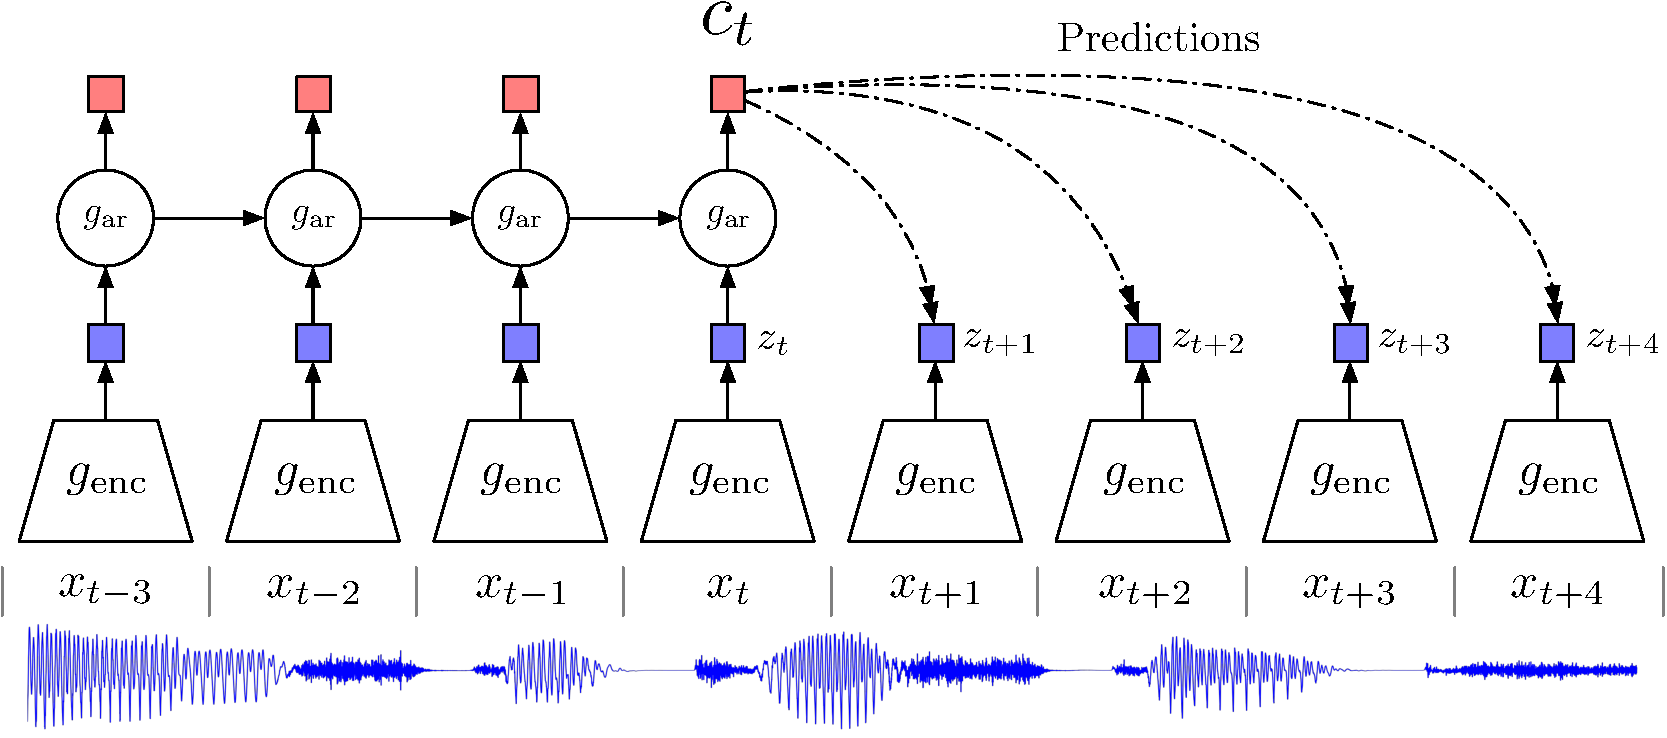
\includegraphics[scale=0.4]{contrastive_repr4.pdf}
    \caption{Image from \citep{oord_representation_2019}. Overview of Contrastive Predictive Coding framework using audio signal as input. }
\end{figure}



Let us see how we train the encoder $g_{enc}$ and the autoregressive model $g_{ar}$.\\